% !TeX spellcheck = en_US
\chapter{Methodology}%

\section{Introduction}%

The proposed method aims to provide a framework for optimizing various parameters of an industrial robot toward a specified objective. By effectively utilizing the redundant degrees of freedom mentioned in Chapter \ref{OBJECTIVE}, this method is applicable to robotic milling operations and WAAM processes. The successful implementation of this methodology improves the robot's overall performance and efficiency, leading to increased productivity in industrial operations. The methodology is broken down into two parts. First, an evaluation of process parameters for a specific tool path with set boundary conditions, and second, an optimization of those boundary conditions to optimize the specific process parameters.

\section{General Methodology for Process Analysis and Evaluation}
\subsection{General Methodology}\label{general}

The flowchart in figure \ref{BasicScore} shows the interdependence of a tool path, the used manufacturing machine, the material, and set boundary conditions. The machine defines general parameters like total working volume, DoF, maximum feed rates, and manufacturing process (additive or subtractive). It can be a 6-axis CNC machine or an 8-DoF industrial robot. The part is referred to as the finished geometry as designed in CAD. The material is a user-defined element from which the part should be manufactured. The elements "Machine", "Part" and "Material" directly influence the toolpath that is necessary for manufacturing. The machine, for example, defines if the spindle or the work piece itself needs to be tilted while machining to achieve the desired geometric features. Further elements like available end-mills, desired depth of cut, machining strategy and operation sequence are regarded as adjacent parameters. 


As the tool path is only a relative movement in regards to the work piece, the user is required to define further parameters before starting the manufacturing process. One example is the positioning of the raw stock material in the machine itself and defining the coordinate system that is used as a reference for the tool center point (TCP). These boundary conditions have to be in accordance with the machine's capabilities and can require extensive knowledge about the machine as well as the performed process.
\begin{figure}[H]
	\centerline{\includegraphics[scale=.6]{figures/BasicScore.png}}
	\caption{Interdependence of various parameters}
	\label{BasicScore}
\end{figure}

One of the other parameters that needs to be defined in the "User-Defined Boundary Conditions" is the positioning or constraining of redundant DoF. One of the simplest cases to illustrate this constraining, is when using a 6-DoF robot for milling operations. In milling, the TCP position is defined by three coordinates, namely X, Y, and Z, as well as the rotation around the X and Y axes. The rotation around the Z-axis needs to be defined manually, as the spindle is rotationally symmetric around that axis. This constraint ensures that the robot maintains a specified pose while performing milling operations. The rotation around the Z axis can, in theory, be set to any arbitrary value but can influence the overall process parameters significantly. In practical applications, this rotation value is limited due to factors like cable routing or joint limits. The same limitations come into play in WAAM where the wire feed system cobmined with the torch position limit the possible orientation.

After the constraints are set and the tool path is generated, various process parameters can be analyzed. Some of the more prominent parameters are the total angular travel of a specific joint or the total angular acceleration. In addition to these numerical values, the user can define a specific importance for the analyzed process parameters and, with a weighting of all available process parameters, calculate an overall score of the determined tool path.

In the following, the elements "Adjacent parameters" and "Material" are omitted as they do not directly impact the optimization of a manufacturing process, as explained in Chapter \ref{OBJECTIVE}. They are hard constraints that define the possible tool path and are not directly related to the redundant DoF. Nonetheless, it is important to note that these adjacent parameters can still offer a significant improvement in areas like cycle time or surface finish of the manufactured part.

%More information regarding the parameters and weights is presented in chapter \ref{pp}.
\newpage
\subsection{Process Parameters}\label{pp}


Table \ref{procesparameters} presents a comprehensive overview of the various process parameters that can be derived from a tool path with defined boundary conditions that is executed by an industrial robot. 


\begin{table}[H]
	\centering
	\begin{tabular}{||l|r||}
		\hline
		Process Parameter & Numerical Form\\
		\hline
		\hline
		\hline
		Angular position of each joint & Time-series\\
		Angular velocity of each joint & Time-series\\
		Angular acceleration of each joint& Time-series\\
		Angular jerk of each joint& Time-series\\
		\hline
		\hline
		Direction changes of each joint& Scalar value\\
		Total travel of each joint& Scalar value\\
		\hline
		\hline	
		
		TCP coordinates (X,Y,Z) & Time-series\\
		TCP velocity (X,Y,Z) & Time-series\\
		TCP acceleration (X,Y,Z) & Time-series\\
		
		
		\hline
		\hline
		Continuous energy usage & Time-series\\
		Total energy usage & Scalar value\\
		\hline
		\hline
		Reachability index & Binary value / Time-series\\
		Singularity Analysis & Scalar value / Time-series\\
		Torch orientation & Time-series\\
		
		
		\hline
		\hline
		
	\end{tabular}
	
	
	\caption{Process parameter and their numerical form}
	\label{procesparameters}
\end{table}

One of the first key parameters is the joint position, which is typically recorded as a one-dimensional array containing the rotational position or extension values of each rotary or linear joint at every time step. This information serves as a basis for determining subsequent parameters such as velocity, acceleration, and jerk. These parameters are important to analyze so that it can be ensured that the joints are not overly strained in the manufacturing process and their service life can be extended as much as possible.
 
In order to prolong the lifespan of an industrial robot, it is crucial to consider the load on individual joints. One important indicator of joint load is the number of direction changes that a joint undergoes during its operation. High-frequency rotation changes can result in significant degradation and loss of precision during manufacturing processes.
This process parameter, known as the number of direction changes, is a scalar value that can be derived from the angular position of each joint. By further analyzing the joint position data, the total travel of a joint can be determined by taking the integral of the joint velocity over time.

Additionally, it can be analyzed whether a velocity change always occurs at the same position and thus introduces wear at the same tooth flank. This results in significant local wear and shortens the lifespan of the joints. 
\newpage
Programs or tool paths that require less total joint travel are generally more desirable. By minimizing the number of direction changes and optimizing the joint travel, the stress and wear on the robot joints can be reduced, thereby extending the overall lifespan of the robot system.

By employing a forward kinematics approach or extracting it directly from the G-code, it becomes possible to determine the position (X Y Z position) and orientation (rotation) of the TCP (Tool Center Point). Additionally, the acceleration and jerk of the TCP can be calculated by taking the respective derivatives with respect to time. These derived parameters, along with the joint positions, are all stored in the form of arrays that capture the temporal changes in their respective values. These parameters can be used to determine how many times a robot will deviate from the proposed tool path and how much deviation in the continuous path mode can be expected.



Estimating the energy usage in industrial robot applications is another crucial aspect that is becoming more important in the current manufacturing environment. One option to accurately estimate energy consumption is to perform a multi-body simulation. For that, it is essential to have a correct 3D model that includes information about the weight and its distribution of the robot joints. Another option is to employ machine learning (ML) approaches or any other intermediate analysis.

Furthermore, in cases where the industrial robot is utilized for WAAM, the power required for welding can be extracted from the G-code by analyzing the duration for which the welding torch remains active. The continuous energy similarly to the other parameters mentioned earlier, is also represented in the form of an array to capture the variations over time.

Total energy usage, measured in kWh, is a key parameter that can be measured directly during the manufacturing process. It provides valuable insights into the overall energy consumption of the industrial robot system. This parameter can be obtained by monitoring the energy usage in real-time or by integrating the time-series data of the continuous energy consumption. By analyzing energy usage, manufacturers can identify energy-intensive processes or operations, optimize energy consumption, and implement strategies to reduce overall energy consumption, leading to cost savings and environmental benefits.

%Alternatively, if direct measurement of energy usage is not available, the energy consumption can be estimated by integrating the time-series data of the energy consumption. This involves summing up the energy consumed at each time-step over the duration of the manufacturing process. Although this estimation method may not be as accurate as direct measurement, it can still provide valuable insights into the overall energy usage.


The reachability index is a binary parameter used to determine the feasibility of executing a program in an industrial robot system. This index indicates whether all the necessary points defined in the tool path are inside the working volume of the robot and can be reached by the robot's TCP. This parameter helps ensure that the robot can physically access all the required positions in the work area. If any point is found to be outside the reachable workspace, it indicates a need for adjustments. Additional factors like cable routing can also influence reachability, even though the endpoints lie inside the working volume of the robot. Wire-feed systems or optical fiber used to transmit a laser can only tolerate a set bending degree. When specifically analyzing the orientation regarding the cable routing, the reachability index can take the form of a time-series that records the deviation of the bending angle of a cable from the optimal angle.


The singularity analysis parameter can be represented either as a time-series or as a single numerical value. It is based on the smallest eigenvalue of the Jacobian matrix, which is calculated using the robot's current configuration. This parameter can be stored in array form, capturing the changes in singularity analysis over time. Alternatively, only the smallest eigenvalue encountered during the entire tool path can be recorded. The analysis of the singularity time-series can be used to optimize non-optimal poses, ensuring that the robot avoids singular configurations that may lead to reduced performance or unexpected behavior.

%Torch orientation is a parameter specific for WAAM. It tracks the tilt angle of the welding torch. For optimal performance is it necessary that the material depositions happens in direction of gravity. In the worst case scenario the welding head is positioned upside down and the welding process is happening against the direction od gravity. The time-series records the deviation of the torch angle from the gravity vector.



Torch orientation is a critical parameter in WAAM. It monitors the tilt angle of the welding torch during the process. To achieve optimal performance, it is essential that the material deposition process always occurs in the direction of gravity. When the welding head is positioned upside down, it represents a worst-case scenario where the welding process takes place against the force of gravity.
When the tilt angle significantly deviates from the gravity vector, maintaining the stability of the molten metal pool becomes more difficult, potentially leading to defects like sagging. 

To ensure the torch orientation is properly monitored, a time-series is used to record the deviation of the torch angle from the gravity vector. Analyzing this information helps identify any deviations or issues that may affect the quality of the deposited material. 


%To ensure safe and efficient operations, both the reachability index and the collision index are evaluated before the G-code program is executed. If all positions in the tool path are reachable and no collision is expected, the G-code is considered safe for production and can be executed. If any issues are identified, adjustments can be made to the program or the robot's configuration to ensure proper reachability and collision avoidance.




Figure \ref{ParamsFlow} visualizes how the different parameters are interconnected. It is clearly visible that all parameters can be derived from the angular position of the joints. This is a clear indicator of the importance of that information. The angular position data provides essential information for analyzing and optimizing the performance of the robot system. By monitoring and analyzing the joint positions, the user can gain insights into various aspects of the robot's operation and make informed decisions to optimize productivity.




\begin{figure}[H]
	\centerline{\includegraphics[width=0.781\textwidth]{figures/Flow.png}}
	\caption{Parameter Flowchart}
	\label{ParamsFlow}
\end{figure}

\newpage

\section{User-Defined Weights and Score Calculation}\label{weights}
\subsection{Local Rating and Global Score}
To assess if a tool path with its boundary conditions is optimal or offers the possibility for improvement, a score or rating value is required that takes the process parameters and their importance into account. 

Determining the relative importance of different parameters can involve subjective judgments, expert knowledge, and consideration of specific manufacturing constraints. For example, in some cases, minimizing joint jerk may be the primary objective, while in others, energy usage may take precedence.

To quantify the performance of a tool path, the user can assign weights or importance factors to each parameter based on their specific requirements. These weights can reflect the relative significance of each parameter in achieving the desired optimum. A weighted sum or scoring method can then be used to evaluate and compare the same tool paths with different constraints based on the aggregated scores of the individual parameters. %The sum of all defined importance values must add up to 1 so that the most optimal tool path has the global score of 100.

It's important to note that the subjective weighing of parameters can vary between different manufacturing scenarios and requires continuous evaluation and adjustment based on changing priorities or goals.

The score of a tool path with its boundary conditions is calculated as shown in table \ref{weighting}. Each process parameter can take a local rating in the range 0-100. 0 being the least optimal, while 100 represents the optimal best-case solution. This value is multiplied by the importance factor and returns the local score. 
All local scores are summed up and result in the overall global score of that specific tool path with corresponding boundary conditions and that specific importance assignment.
The sum of all defined importance values must add up to 1 so that the most optimal boundary conditions lead to a global score of 100.


\begin{table}[H]
	\centering
	\begin{tabular}{||l|r|r|r||}
		Process Parameters & Local rating & Importance & Local score\\
		\hline
		\hline
		\hline
		
		Process Parameter 1 & 74 & 0.5 & 37\\
		Process Parameter 2 & 34& 0.1&3.4\\
		Process Parameter 3& 65& 0.1&6.5\\
		Process Parameter 4& 22&0.3&6.6\\
		\hline
		\hline
		\hline
		Global Score& & &53,5\\
		\hline
		\hline
	\end{tabular}
	
	\caption{Calculation of a tool path score}
	\label{weighting}
\end{table}


\subsection{Local Rating Calculation}\label{LRC}
Calculating a local rating is not a straight-forward approach. The first problem is that based on a singular value like "direction changes," it is not possible to determine a local rating as it is not clear if that value is close to optimal or far from it.
The solution to this problem is to calculate the tool path with different boundary conditions or constraints, like rotation around the C-axis, and compare the different results.
Figure \ref{Localscore} shows how a local score can be calculated by means of variation. Each variation leads to a different number of direction changes in joint 1. The local score is calculated by essentially applying a Min-Max scaler.

\begin{figure}[H]
	\centerline{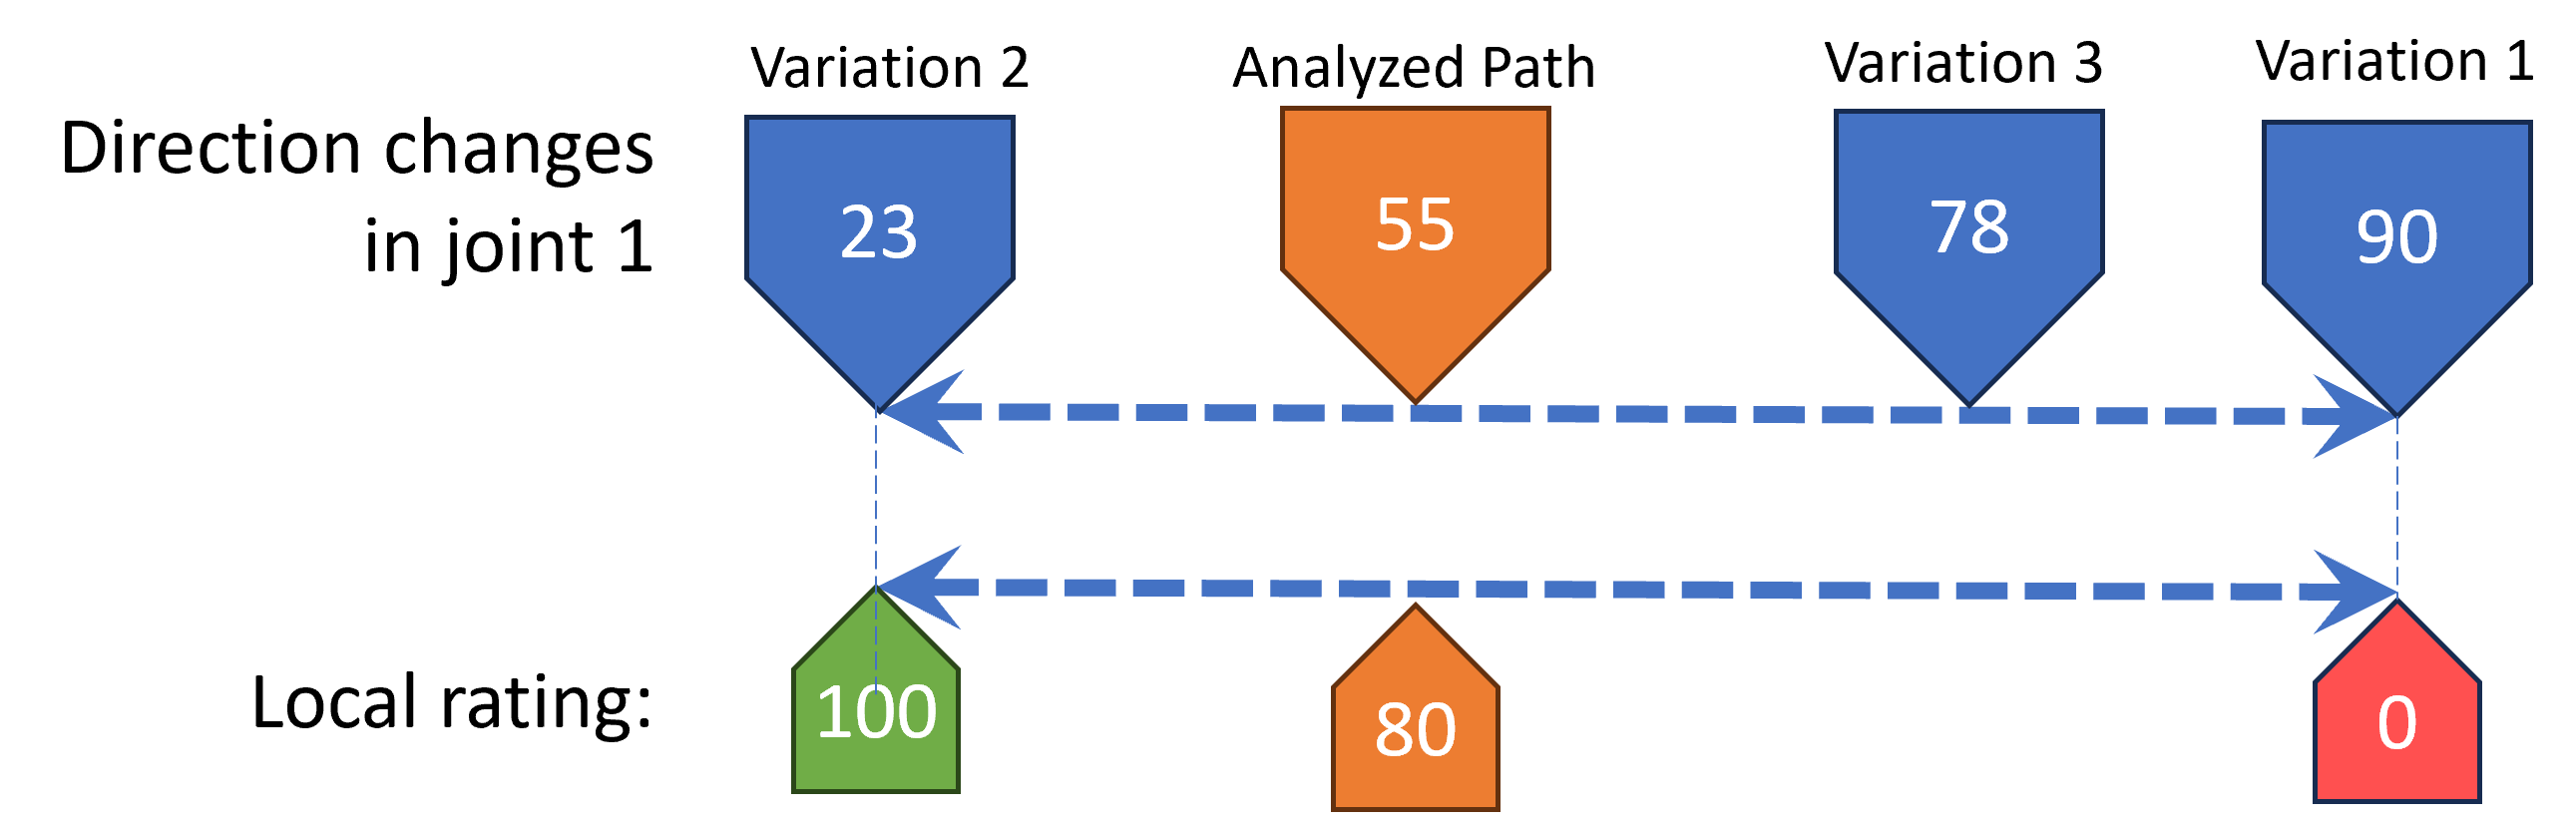
\includegraphics[width=0.8\textwidth]{figures/localscore.png}}
	\caption{Calculation of the local score trough variation}
	\label{Localscore}
\end{figure}

It is important to note that performing more variations before calculating the local sore will increase the accuracy of this approach. If only a few variations are performed, it is possible that only variations with similar outcomes will be found, which can skew the result significantly.

Another factor that needs to be analyzed is whether the variations in the boundary result in local scores that exceed a certain standard deviation. Figure \ref{lowstd}, shows how a local score of 66 is calculated despite the presence of very small absolute differences. In this case, the standard deviation is only 0.37. Figure \ref{highstd} demonstrates how the same local score of 66 is calculated even though the absolute differences are significantly higher. Here, the standard deviation is 22.36. Only if the standard deviation exceeds a set threshold should the local score be used as input for the global score. In cases where the standard deviation criteria is not met, the corresponding process parameter should be omitted from the global score calculation.

\begin{figure}[H]
	\centerline{\includegraphics[width=0.8\textwidth]{figures/lowstd.png}}
	\caption{Variation with low standard deviation}
	\label{lowstd}
\end{figure}

\begin{figure}[H]
	\centerline{
\includegraphics[width=0.8\textwidth]{figures/highstd.png}}
	\caption{Variation with high standard deviation}
	\label{highstd}
\end{figure}

 
\subsection{Information Extraction form Time-Series Data}\label{extraction}
It is important to note that for a local score computation, as mentioned in Chapter \ref{LRC}, a time-series needs to be transformed into a scalar value. This can either be done by directly transforming the time-series like, for example, summing up all values or performing a subsequent analysis. As each time-series is capturing different physical phenomena, each one requires an individual process for transforming into a scalar value.
\newpage




\section{Information from Angular Position}
The angular position of a joint by itself does not provide much information from which much qualitative analysis can be performed. But by adding information, like a temporal component, it can serve as a significant information source. 

Figure \ref{agularstuff} visualizes what information needs to be added to enhance the information content of process parameters that are directly related to the angular position of joints.

\begin{figure}[H]
	\centerline{\includegraphics[width=0.8\textwidth]{figures/angularstuff.png}}
	\caption{Additional Information for angular position of each joint}
	\label{agularstuff}
\end{figure}



The first additional piece of required information is the temporal element, which specifies the time when a joint is supposed to be in what rotational position. This information can either be recorded in equidistant time steps as shown in figure \ref{equi} on the left or adapted to only record the change of position as shown on the right. Recording only the change of position is not optimal as it does not correspond to the physical system, where the position cannot significantly change from one time step to the next. Additionally, it is not defined with which rotational velocity the joint needs to change position. On the other hand, continuous recording in small equidistant time steps can result in significantly more recorded values and thus, a longer time-series.

Figure \ref{equi} shows the rotational position of a rotary joint in radians recorded with equidistant steps as well as a time-series where only the destination positions and the associate times are recorded.


\begin{figure}[H]
	\centerline{
\includegraphics[width=1\textwidth]{figures/equionchange.png}}
	%\caption{Time-series of a rotary joint with equidistant time steps}
	\caption{Two option for recording the joint position in a time-series}
	\label{equi}
\end{figure}

%\begin{figure}[H]
%	\centerline{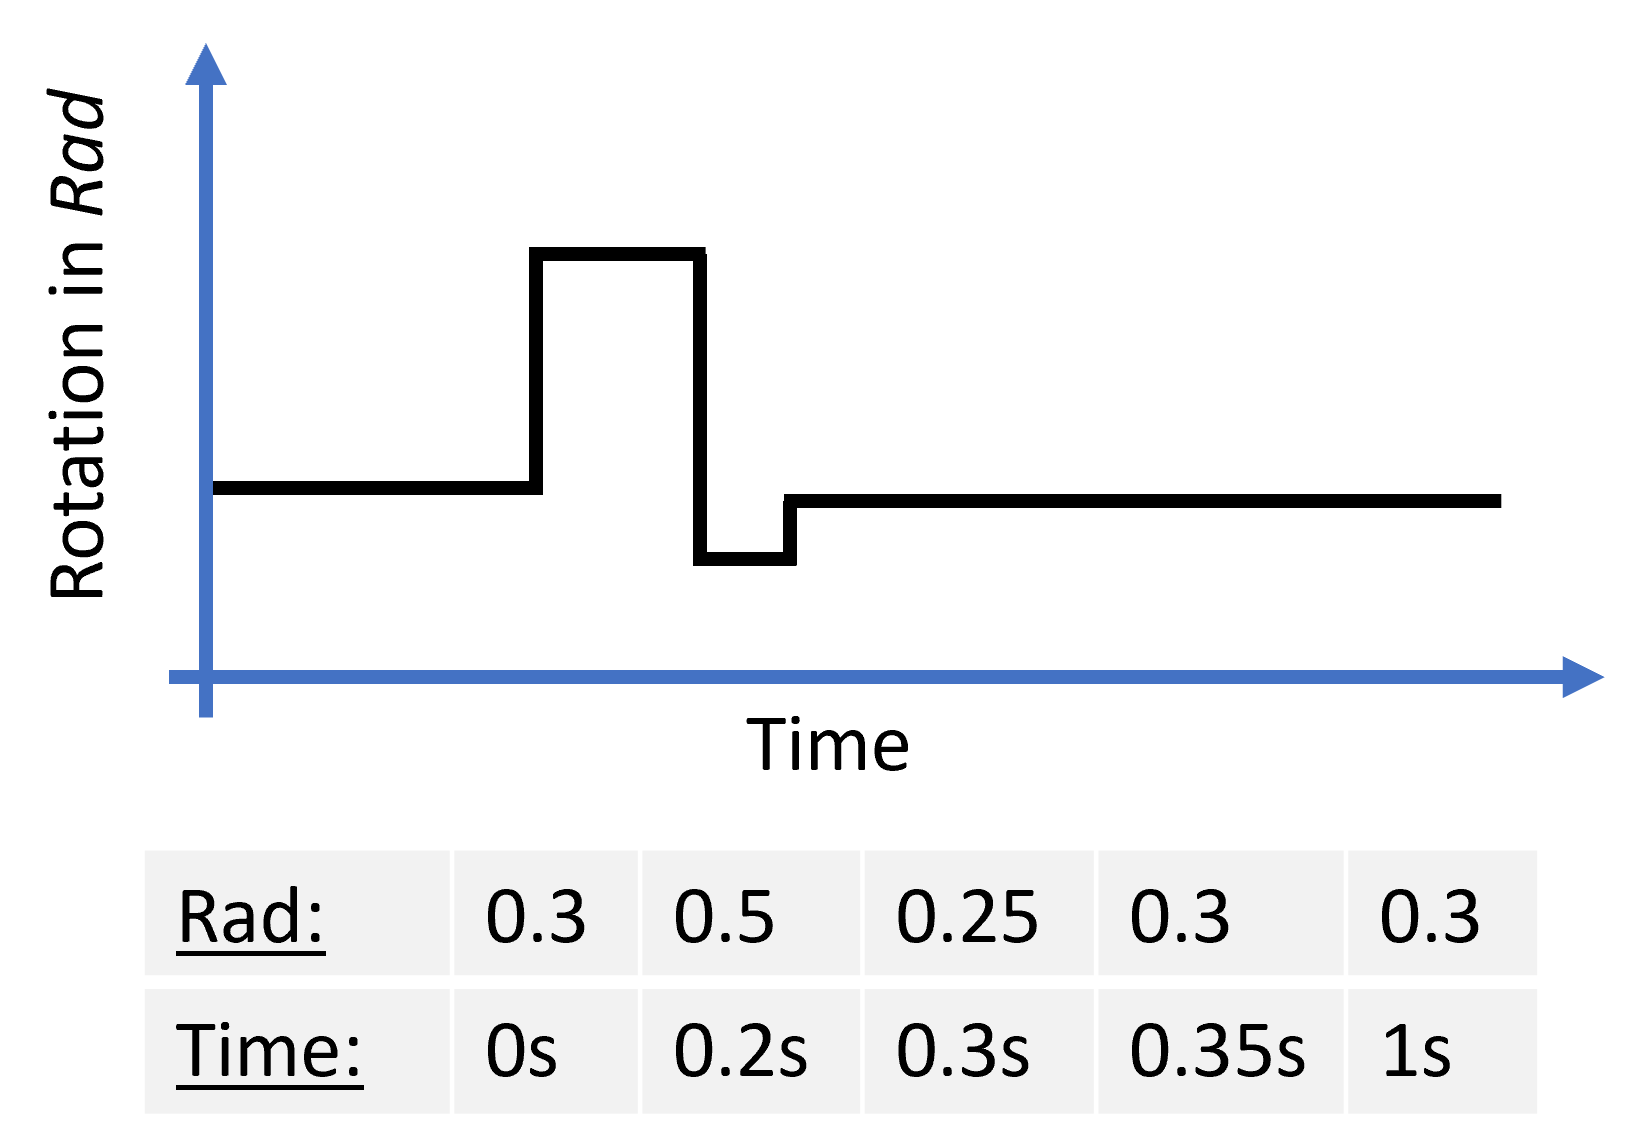
\includegraphics[width=0.5\textwidth]{figures/onchange.png}}
%	\caption{Time-series of a rotary joint with only the recorded end positions}
%	\label{onchange}
%\end{figure}

\subsection{Total Joint Travel and Direction Changes}
Parameters that can be analyzed without any additional information are the number of direction changes as well as the total travel of a joint. The total travel is easily obtained by subtracting the position from two adjacent recorded points and summing up the absolute value. Additionally, more information can be extracted by summing up, for example, the clockwise and anti-clockwise rotations individually. By combining the absolute values of these, the total travel of that joint is calculated.

Figure \ref{travel} gives a visual representation of how the total travel can be calculated. Summing up the length of the green arrows results in the total forward rotation, while the sum of the length of the orange arrows is the backward rotation.

\begin{figure}[H]
	\centerline{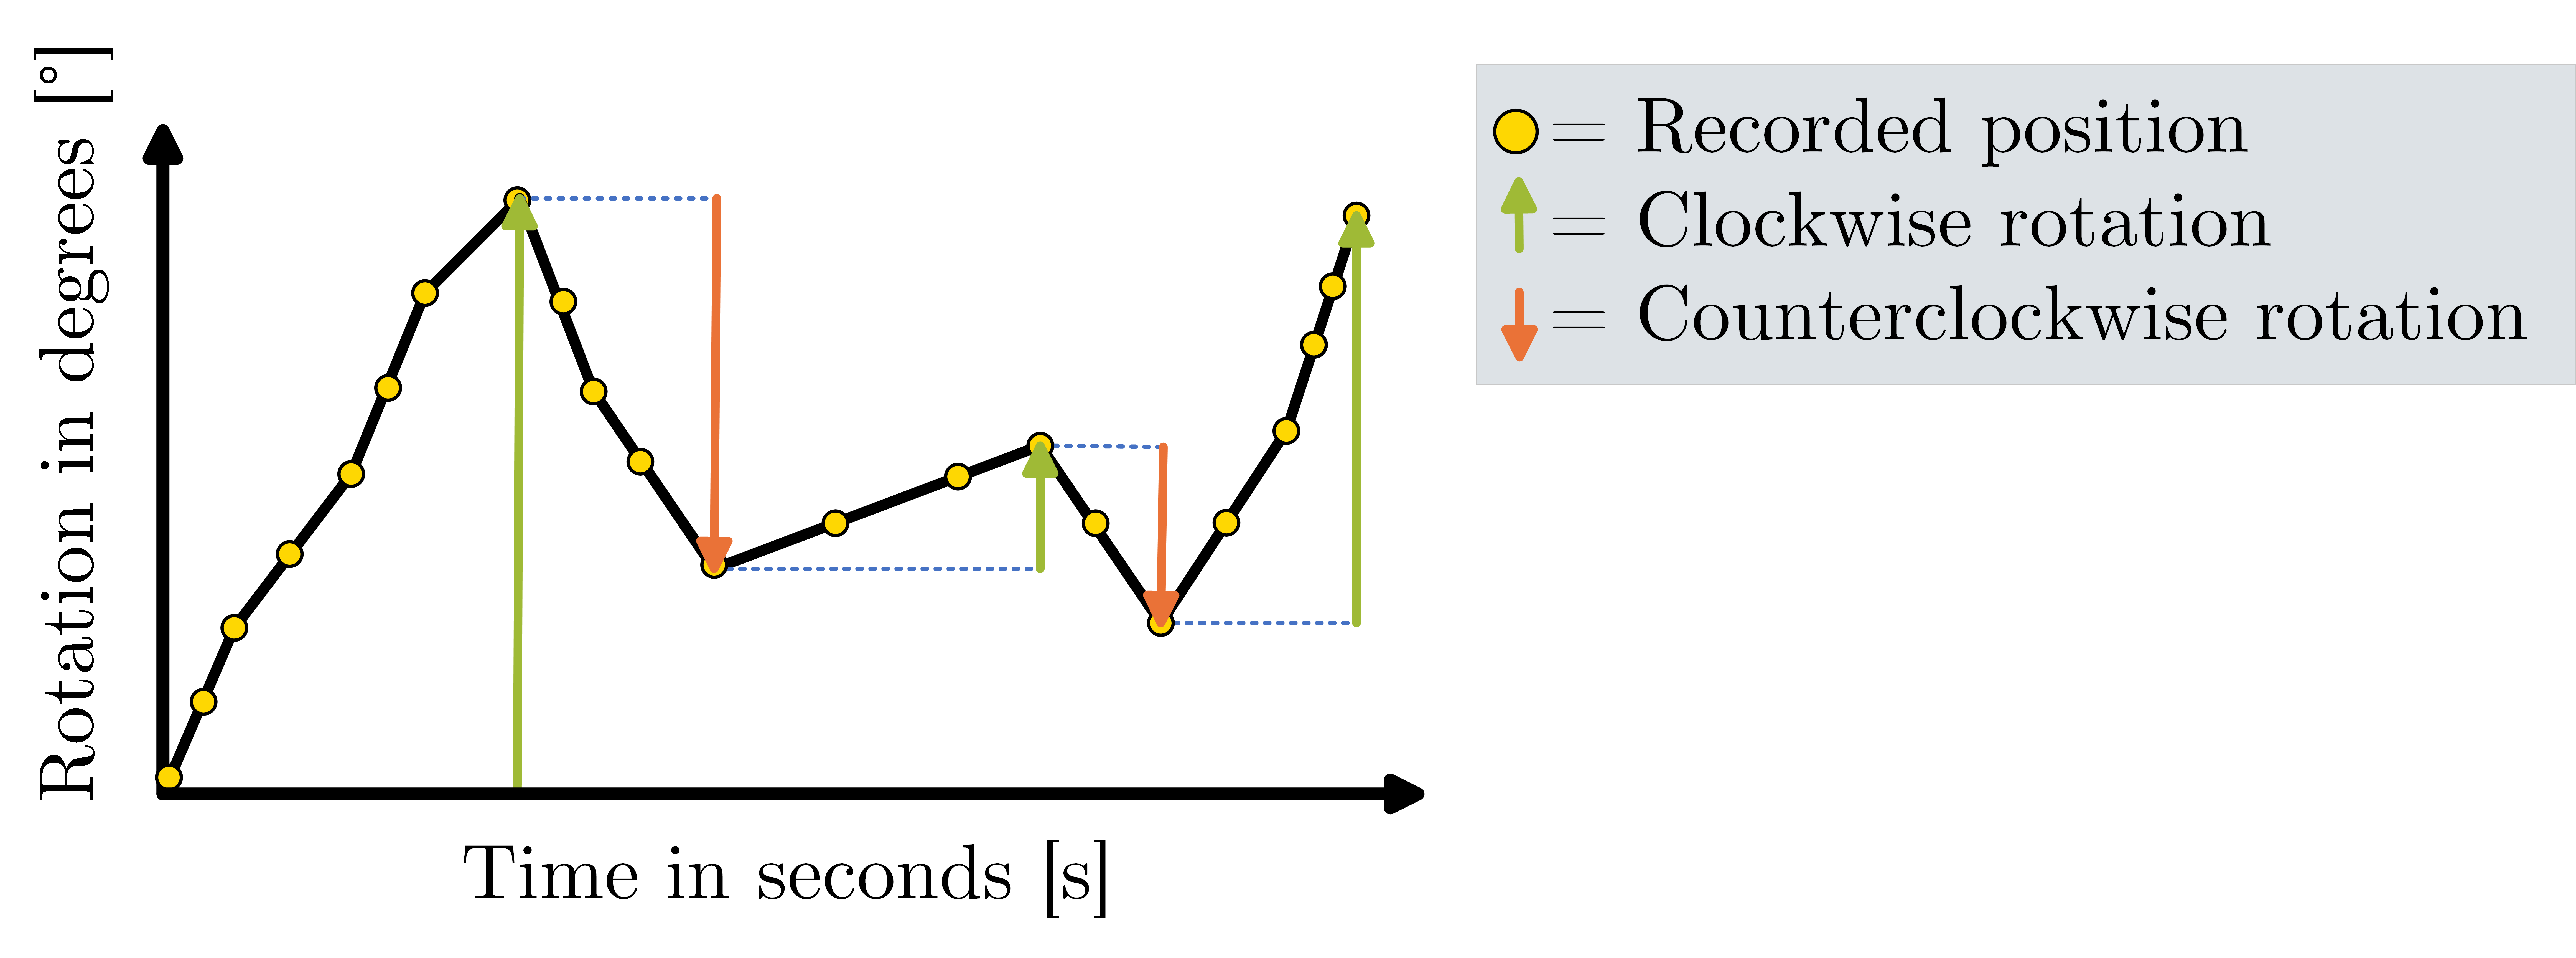
\includegraphics[width=0.5\textwidth]{figures/travel.png}}
	\caption{Summing up the rotation in the clockwise and anti-clockwise direction }
	\label{travel}
\end{figure}

The number of direction changes is a parameter that can also be determined by just analyzing the joint position without having the temporal information. This value can be determined by finding all points where the position before and after is either smaller or larger. 
But this method is not applicable to points where multiple positions are recorded at the same value right after each other.

The solution to that problem is to introduce a tracking value that indicates if the previous change in direction of two adjacent positions was either up or down. If the direction of two positions is different from the tracking value, the direction change counter is incremented by 1. If the direction is the same as the previous points or neutral, which means that two positions were identical, the direction change counter and tracking values are not changed.

Figure \ref{dirchange} gives a visual representation of where the direction-change-counter is incremented.

\begin{figure}[H]
	\centerline{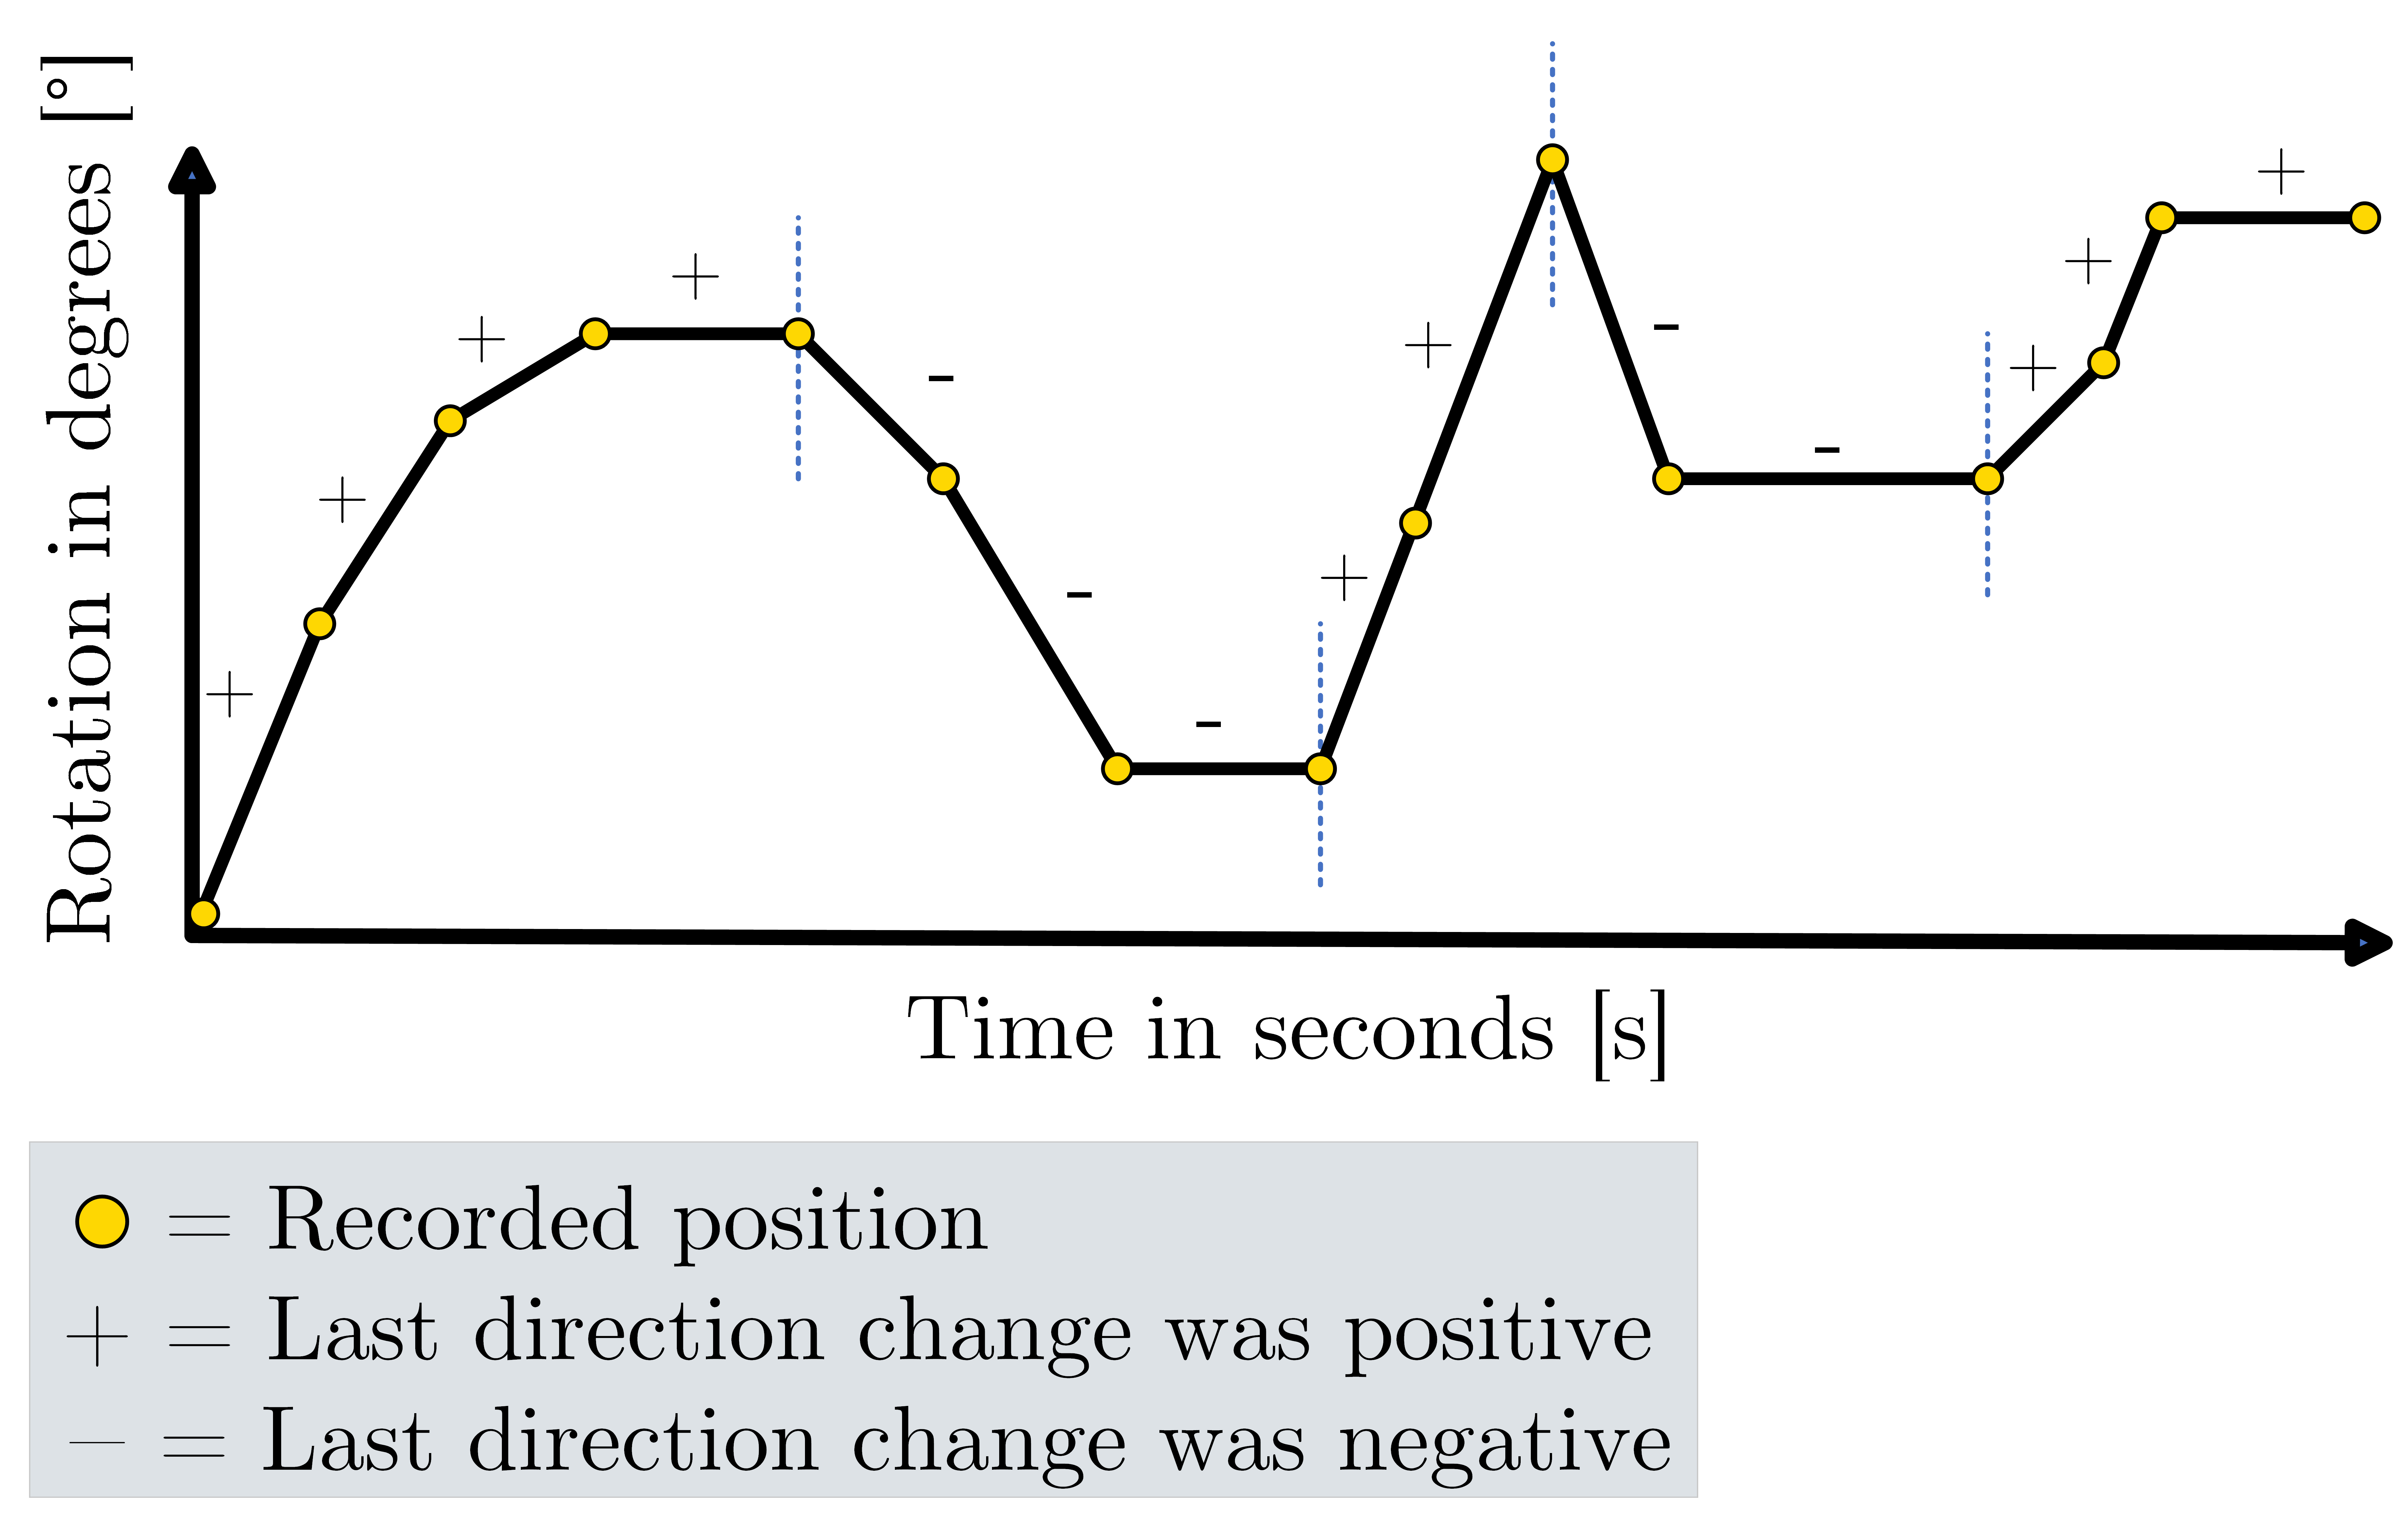
\includegraphics[width=0.8\textwidth]{figures/dirchange.png}}
	\caption{Calculating direction changes from a time-series}
	\label{dirchange}
\end{figure}

The counter of the direction changes and total travel of each joint are the values that are then transformed into a local sore as explained in Chapter \ref{LRC} and then multiplied with an importance factor to result in the local score. The direction changes can either be summed up over all joints or specifically grouped.  

Table \ref{exampleDirTravel} gives an example of how a global score can be calculated based only on the number of direction changes and total travel. In this example, the highest importance is assigned to the direction changes of joint 1. Direction changes in joints 2 to 6 are grouped together. Further, the total travel in joint 4 is also explicitly weighted, while the total travel of the other joints is grouped together. It is important to note that only the local score is multiplied by the importance factor, not the actual counted direction changes or total travel. This is why the values lie in an interval between 0 and 100. As the direction changes in joint 1 have a high local score and a high importance factor, the overall global score is also very high. This again indicates the significance of setting the imortance factor in accordance with the desired outcome. 


\begin{table}[H]
	\centering
	\begin{tabular}{||l|r|r|r||}
		Process Parameters & Local rating & Importance & Local score\\
		\hline
		\hline
		\hline
		
		Direction changes in joint 1 & 95 & 0.7 & 66.5\\
		Direction changes in joint 2-6 & 45& 0.1&4.5\\
		Total travel in joint 4& 34& 0.1&3.4\\
		Total travel in joint 1-3 and 5-6& 46&0.1&4.6\\
		\hline
		\hline
		\hline
		Global Score& & &79\\
		\hline
		\hline
	\end{tabular}
	
	\caption{Calculation of a score regarding only direction changes and total travel}
	\label{exampleDirTravel}
\end{table}

In some cases, it is not possible to reduce the number of direction changes by adapting the boundary conditions. But having the same number of direction changes does not make two time-series identical. Figure \ref{dirchangeSTD} shows how two time-series have the same number of direction changes but have significantly different characteristics. To differentiate these cases, a value corresponding to the standard deviation can be employed. Tool paths that result in frequent and temporally close-positioned direction changes are generally not advisable. 


This factor can be combined with the direction changes to form one parameter. This is done by dividing the direction changes by the standard deviation before calculating the local score by means of variation. Few direction changes with a high variance will lead to a low number, which is opposed by many direction changes with a low variance.

\begin{figure}[H]
	\centerline{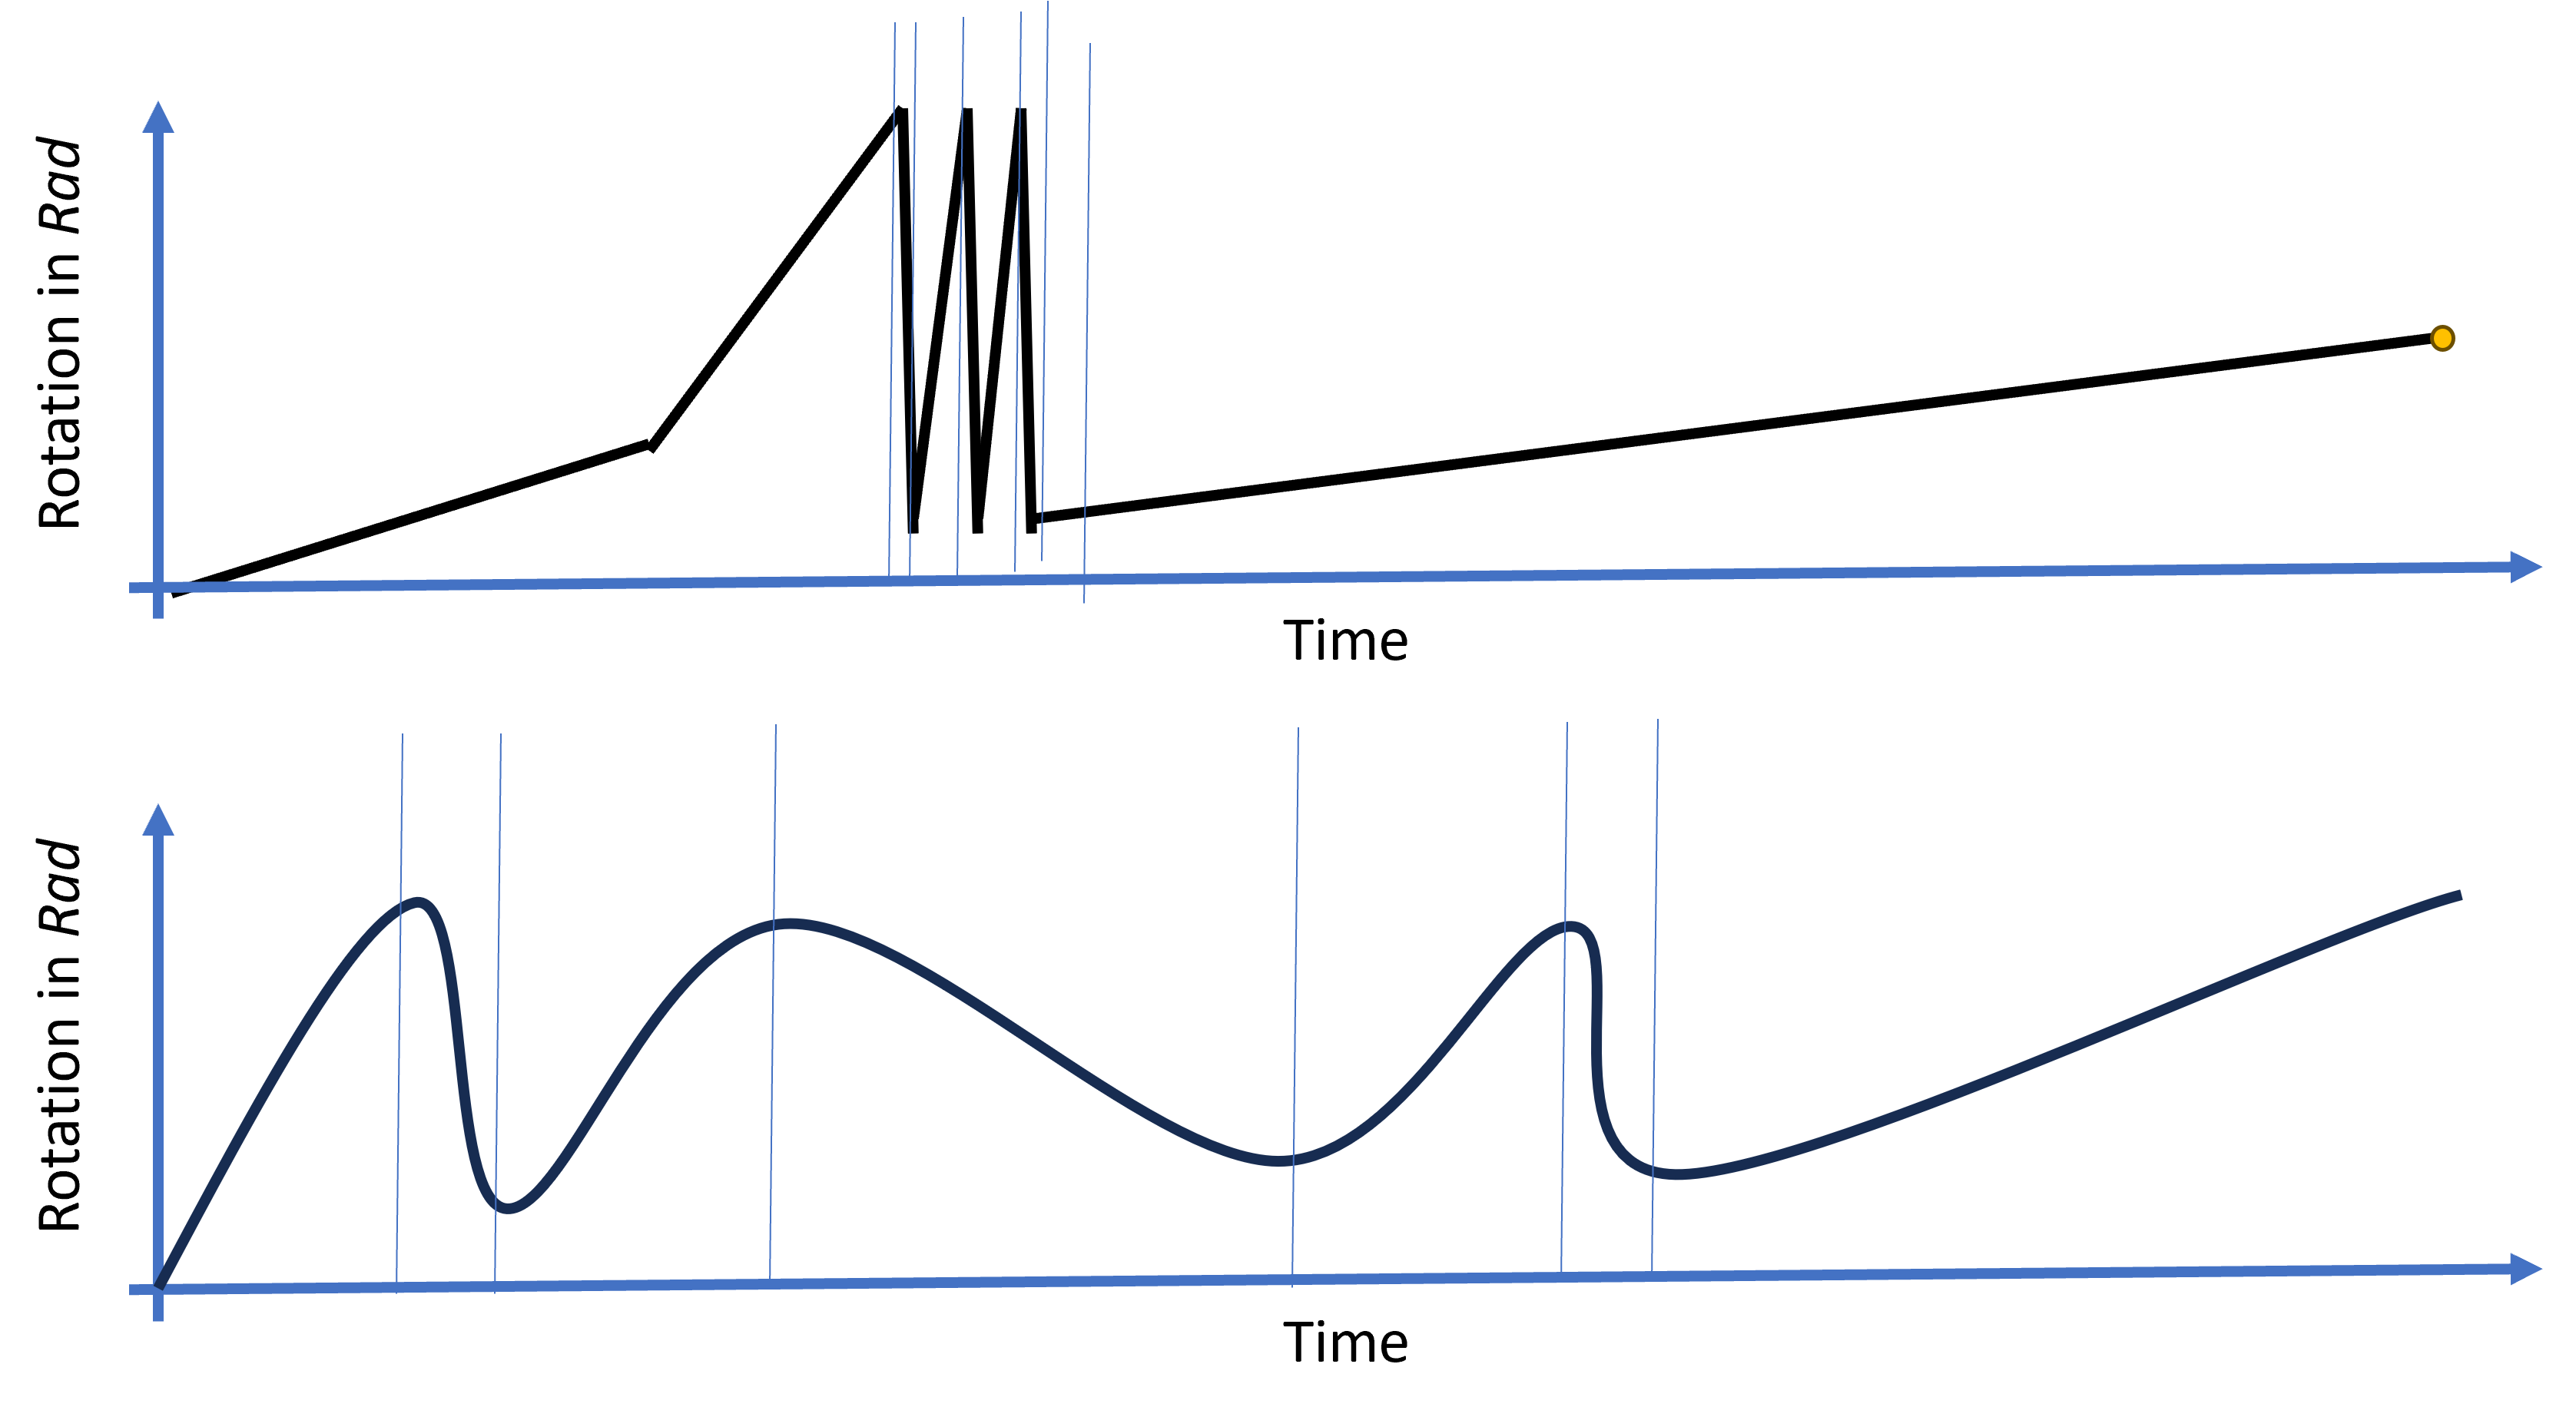
\includegraphics[width=0.7\textwidth]{figures/DirSTD.png}}
	\caption{Two Time-Series with equal number of direction changes but different characteristics}
	\label{dirchangeSTD}
\end{figure}

\subsection{Rotation Limits}\label{RotLim}
Further, a simple analysis regarding the rotational limits can be performed, for which two different values need to be known. The first one is the physical limit that a joint can not exceed. Trying to drive the robot joint past that point can result in significant damage. The second value are possible soft limits that exist to prevent the joint from over-rotation into its physical limits. To validate if any rotational positions come close to the limits or are exceeded, a simple comparison of all the values can be made. If necessary, additional limits can be defined in cases where it is known that a joint is most stable in a specific range. After a tool path with set boundary conditions is defined, the joint angles can be analyzed and a simple comparison can be made. If the joint positions exceed the soft limits or deviate too much from their desired orientation, a "No-Go" exception is issued. The analysis of the rotation limits does not contribute to the calculation of the global score but rather serves as a validity analysis to determine if the movement necessary for the toolpath is physically possible.
\newpage
\subsection{Velocity, Acceleration and Jerk of the Joints}
To specifically analyze the rotational velocity, acceleration and jerk of the joints, a time derivative needs to be performed. After that, simple comparisons of the time-series values are enough to determine whether the maximum capabilities of the motor driving the joint are exceeded.

Figure \ref{velo} shows how the velocity aspect can be transformed into a scalar value that can be used for a local score calculation. First, the joint velocity is obtained by taking a time derivative of the joint position. Then it is analyzed for how long the absolute velocity exceeded a certain threshold value. In the example, the threshold is set at 80\%. Further, it is possible to add multiple thresholds and weigh them exponentially in relation to each other. The combined result is then used as a local score.

\begin{figure}[H]
	\centerline{\includegraphics[width=1\textwidth]{figures/veloy.png}}
	\caption{Calculating velocity from the joint position over time}
	\label{velo}
\end{figure}

It is also possible to define if a short but significant peak over the threshold values is more desirable than a constant but small overstep. Figure \ref{peaklong} gives a visualization of these two cases.

\begin{figure}[H]
	\centerline{
\includegraphics[width=1\textwidth]{figures/peaklong.png}}
	\caption{Overstepping the threshold value}
	\label{peaklong}
\end{figure}

In the former case, where peaks are more desirable, it is enough to count the time-steps where the threshold was overstepped. If the avoidance of limits is the first priority, it must be analyzed how close the velocity, acceleration, and jerk came to the maximum limit. The simplest case however, is to just simply square all values and sum them up. By employing this method, no threshold boundaries have to be defined, and high peaks will influence the resulting value more than small constant values.

In the case that the velocity exceeds the maximum velocity, a "No-Go" exception must be thrown as that movement is not possible. The same rating principle is applicable to acceleration and jerk. The derivative of the velocity returns the acceleration, and the next derivative returns the jerk. Individual limits and thresholds can be set to calculate how optimal the robot's movement is. In cases where the maximum acceleration or jerk is exceeded, a "No-Go" error is also thrown.


Table \ref{VAJ} shows the calculation of a global score with a weighting that prefers low acceleration in joint 2 and accepts high velocity in all joints. The acceleration in joint 1 and 3-6 are also of low importance. The jerk is completely omitted from the rating.


\begin{table}[H]
	\centering
	\begin{tabular}{||l|r|r|r||}
		Process Parameters & Local rating & Importance & Local score\\
		\hline
		\hline
		\hline
		Velocity in Joints 1-6& 45& 0.1&4.5\\
		Accelerations in Joint 2& 90 & 0.8 & 72\\
		Accelerations in Joint 1 and 3-6 & 15& 0.1&1.5\\
		Jerk in joints 1-6& 4& 0&0\\
		
		\hline
		\hline
		\hline
		Global Score& & &78\\
		\hline
		\hline
	\end{tabular}
	
	\caption{Calculation of a score regarding only velocity, acceleration and jerk}
	\label{VAJ}
\end{table}


\section{TCP Coordinates, Velocity and Acceleration}\label{CVA}
As mentioned in Chapter \ref{pp}, with the help of a forward kinematics approach it is possible to determine the X-Y-Z coordinates and orientation of the TCP. Alternatively this information can also be directly extracted from the G-code.

By calculating the time derivative of the positions, the velocity of the TCP can be determined, and subsequently, the acceleration can be obtained as well. These two parameters play a crucial role in milling applications, particularly when the goal is to fabricate precise corners. It is important to note that both robotic systems and CNC machines have limitations on their acceleration capabilities. As highlighted in Chapter \ref{CPM}, these limitations result in slight deviations occurring in the path, especially at corners. These deviations occur due to the inability of the systems to instantaneously change their velocity or direction. Consequently, the path followed by the TCP will not be perfectly smooth and will exhibit minor variations in the corners.


To quantitatively analyze the magnitude and frequency of these deviations, it is crucial to examine the endpoints of the linear toolpath as defined in the G-code. When the endpoints are aligned, it indicates that no deviation from the desired toolpath is expected. However, when there is a misalignment between the endpoints, it indicates that a deviation is expected.

Figure \ref{devi} gives a visual example of the position in th X-Y plane that the robot needs to pass. The expected deviation is shown in red.

\begin{figure}[H]
	\centerline{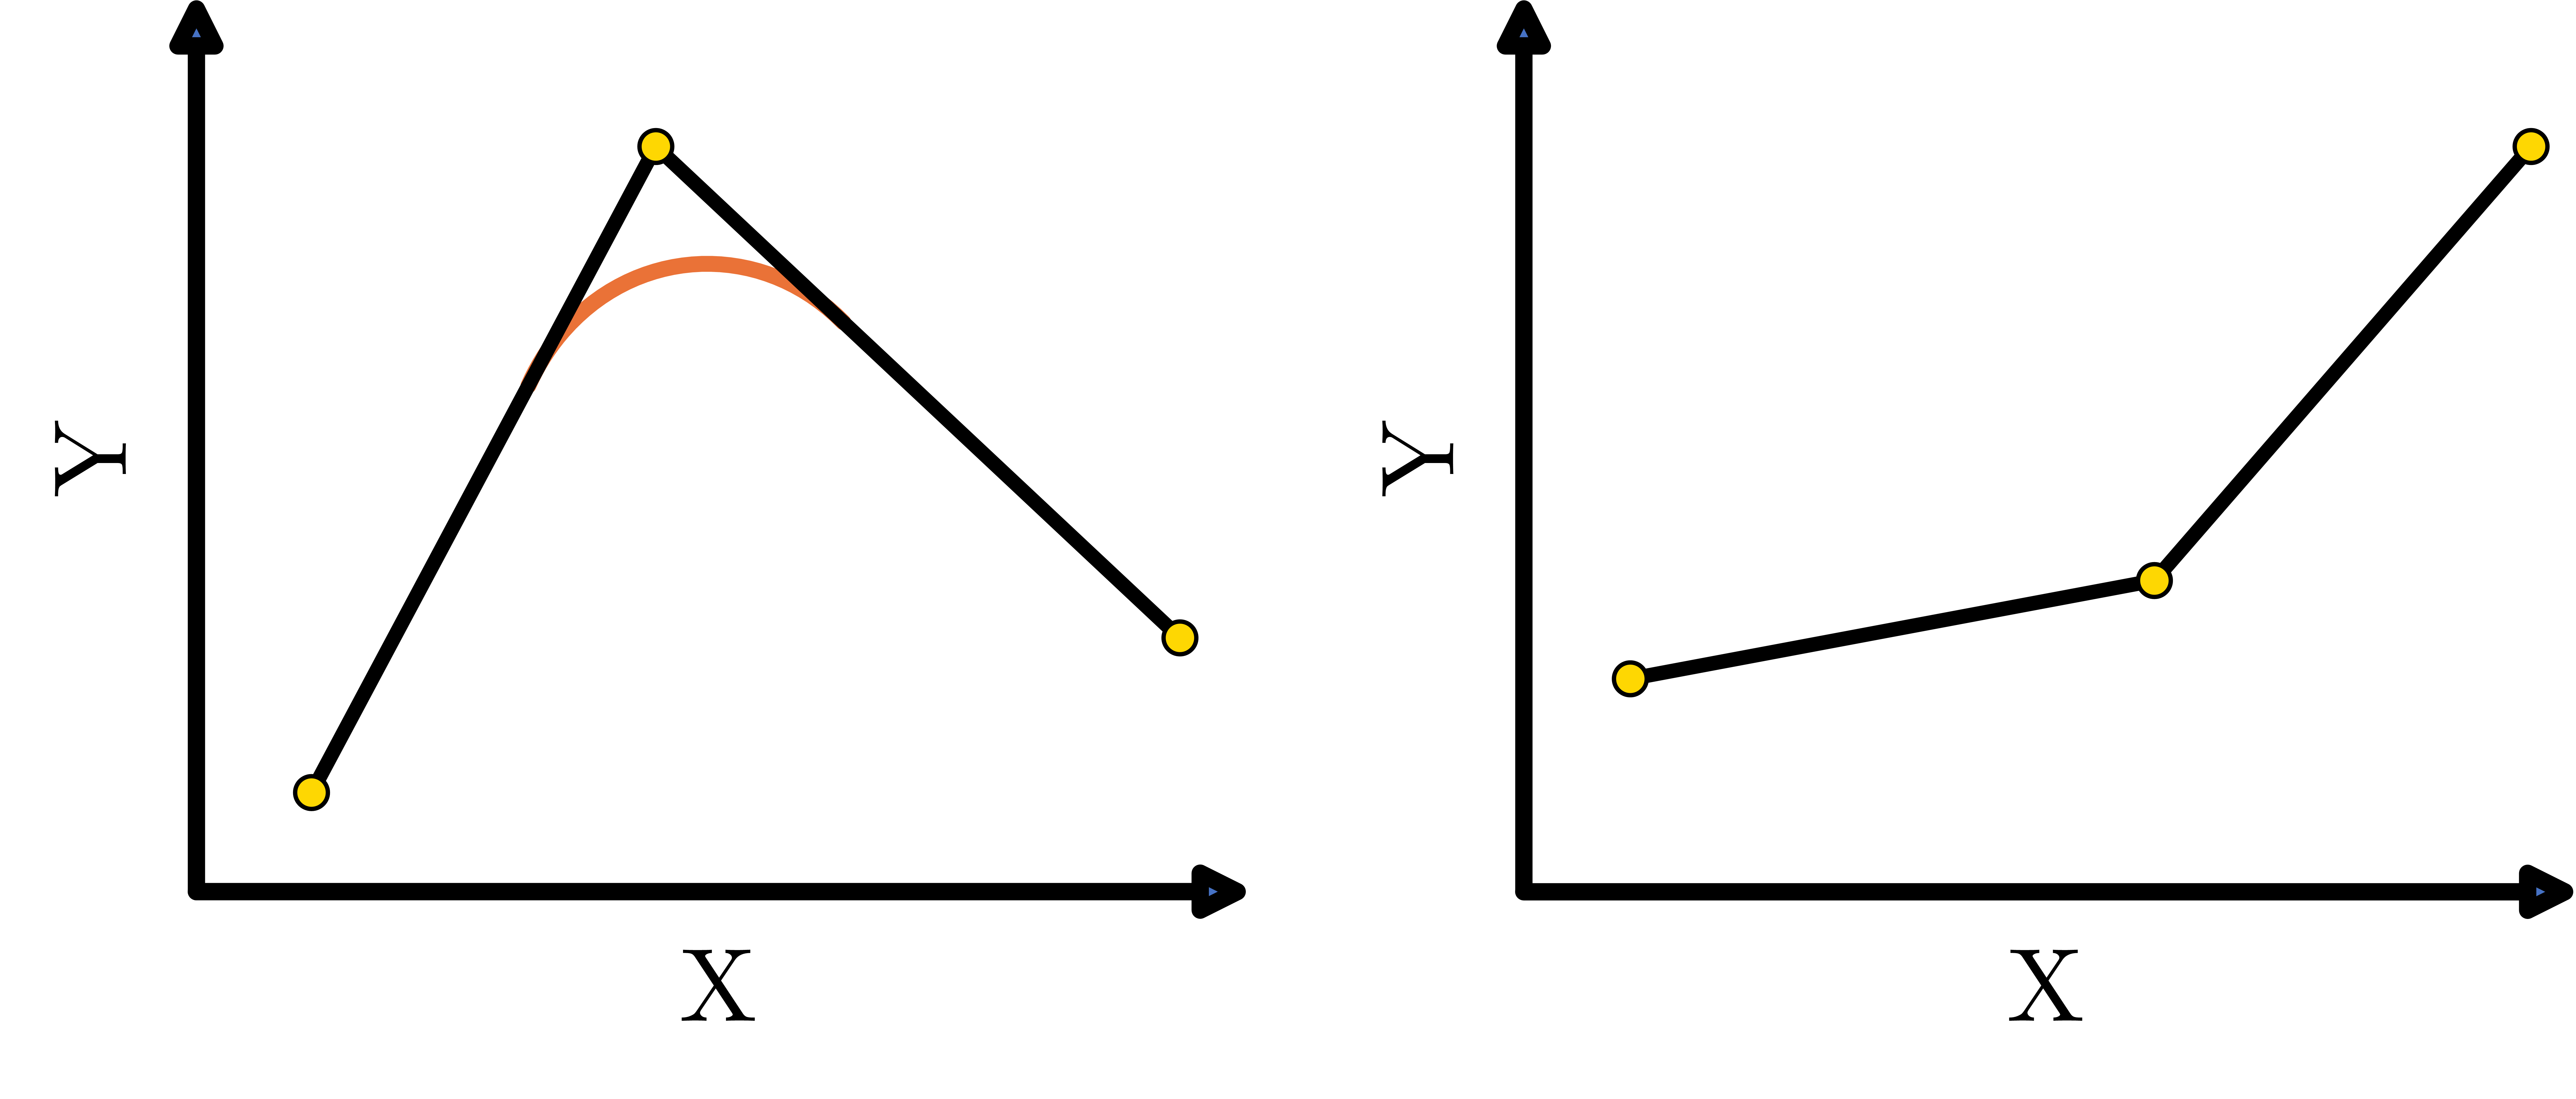
\includegraphics[width=.651\textwidth]{figures/uber.png}}
	\caption{Deviation of of the TCP from the actual toolpath}
	\label{devi}
\end{figure}

To obtain a qualitative estimate of the total deviation, it is necessary to analyze the individual velocity vectors that characterize the toolpath. When the velocity vectors are perfectly aligned, it indicates that no deviation is expected. However, as the angle between two consecutive velocity vectors increases, the deviation also increases.

To quantitatively represent this information, the sine of each angle can be calculated and summed. An angle of 0 or 180 degrees will return 0, while an angle of 90 degrees will return 1. This scalar value provides an indication of the overall magnitude of the expected deviation.

Furthermore, it is essential to consider the magnitude or speed of the velocity vectors. In the case of sharp corners with high velocities, the deviation is expected to be more significant compared to corners with lower velocities. To account for this, the result obtained from the sine calculation can be multiplied by the smaller of the two velocities.

This analysis is helpful for the operator to define more optimal machining strategies but is not related to the optimization with the redundant DoF.

In the context of WAAM, the acceleration of the welding torch can have a significant impact on the process. This is particularly true when using CMT technology, which involves wire retraction, as discussed in Chapter \ref{CMT}. A sharp acceleration of the welding torch can lead to unintended drop detachment and imprecise drop placement. This phenomenon can negatively affect the quality and accuracy of the additive manufacturing process, resulting in defects and deviations from the desired geometry.

However, it is important to note that this issue, similar to the deviation in the toolpath as discussed earlier, is not something that can be directly optimized by simply setting specific boundary conditions. 


THIS WHOLE PARAGRAPH IS USELESS !!


THIS WHOLE PARAGRAPH IS USELESS !!


THIS WHOLE PARAGRAPH IS USELESS !!



\section{Energy Usage}
Energy usage is one of the most important factors in manufacturing today. By carefully selecting optimal boundary conditions, the robot can avoid unnecessary and energy-intensive movements. The energy usage can be analyzed in two different ways. First, there is the continuous energy analysis where each movement can be attribute to a specific energy consumption. Secondly, there is to option for considering the overall energy requirement spanning the entire manufacturing process. This provides a holistic perspective on energy utilization. 

\subsection{Continuous Energy-Usage}
One of the simplest approaches to track energy consumption is by monitoring the velocity and acceleration of individual joints. The energy demand can be divided into two parts: the rotation of a joint with a set velocity and the acceleration of the joint.

To calculate the energy consumption of each joint, the time-series of joint velocity can be multiplied by an average energy consumption value for that specific joint. The same principle applies to the time-series of joint acceleration. By summing up these resulting time-series, an energy consumption time-series for each joint can be obtained. Adding up the time-series of all joints gives the overall energy consumption of the robot. Table \ref{scalers} gives exemplary  values for the scaling factors.\newline


\begin{table}[H]
	\centering
	\begin{tabular}{||l|r|r||}
		Joint Nr.  & Velocity Scaling in \(\frac{\si[per-mode=symbol]{\kWh}}{\si[per-mode=symbol]{\m\per\sec }}\)& Acceleration Scaling in \(\frac{\si[per-mode=symbol]{\kWh}}{\si[per-mode=symbol]{\m\per\sec\squared }}\) \\
		\hline
		\hline
		\hline
		Joint 1	& 0.1 & 0.5\\
		Joint 2	&  0.4& 0.3 \\
		Joint 3	& 0.3& 0.2\\
		...& ...& ...\\
		
		\hline
		\hline
	\end{tabular}
	
	\caption{Average scaling factors for energy calculations}
	\label{scalers}
\end{table}


The main advantage of this approach lies in its simplicity. However, its main drawback is the potential inaccuracy due to working with an average scaling value. If this value is calculated by averaging all possible positions, but only a few are actually traversed by the robot, significant differences may arise.


To overcome these limitations, more sophisticated approaches are required. For instance, implementing multi-body simulations in the CAM software allows for a direct analysis of the precise amount of energy needed for a robot to transition between poses. This method necessitates accurate modeling of weight distribution but yields highly precise results. However, it's important to note that this implementation may require significant computation time.


Another option to consider is utilizing a ML approach for calculating energy consumption during transitions between discrete poses.  By employing a supervised learning technique, where the input data includes the current pose (joint positions and velocities) as well as the target pose, an ML model can be trained to predict the energy required for each transition. This approach offers the advantage of leveraging ML algorithms to provide accurate energy consumption estimates in a more efficient manner. However, it is important to acknowledge that generating high-quality training data and training the ML model can be time-intensive processes.
Figure \ref{ENERGYOPTIONS} shows the three mentioned options with their main requirements. It is important to note that these examples do not covet all possibilities to solve this problem.

\begin{figure}[H]
	\centerline{\includegraphics[width=.8\textwidth]{figures/ENERGYOPTIONS.png}}
	\caption{Exemplary methods for energy usage calculations}
	\label{ENERGYOPTIONS}
\end{figure}

After the time-series for the energy consumption is obtained, it is possible to find peaks and relate them to specific movements. Based on the optimization goal, it is also possible to set analogue threshold values as mentioned in chapter \ref{CVA}, to optimize for a constant energy consumption.


WAMM GCODE
 
\subsection{Total Energy-Usage}
When the objective is to obtain a single scalar value for energy consumption, the same processes described in the previous chapter can be employed, and the values from the time series can be summed up.

However, in cases where the temporal information in energy consumption is considered irrelevant, alternative machine learning approaches can be implemented. For instance, Recurrent Neural Networks (RNNs) can be utilized, which have the ability to take a whole time series as input and return a scalar value representing the total energy consumption. RNNs are capable of capturing dependencies and patterns in sequential data, making them suitable for modeling the energy consumption over time. By training an RNN model using a time series dataset, it can learn to predict the total energy consumption based on the given input. But just as with most ML approaches, this method requires significant upfront effort and time for generating training data and training itself.


\section{Reach, Singularities, Torch Orientation}
In the following, the robot poses with respect to reach, singularity avoidance, and torch orientation is discussed. These are essential factors in ensuring successful and efficient robotic operations.
\subsection{Reach} 

As mentioned in Chapter \ref{pp}, the analysis of the reachability index can be done in multiple formats. The first format involves a simple analysis to determine if all the points that the robot needs to traverse, lie within its work volume  without any collisions occurring with itself or exceeding the hard joint limits. This aspect is closely related to the joint limits, as discussed in Chapter \ref{RotLim}. Further it is necessary to analyze that no collision of the robot with the piecework occurs. Ensuring that the robot's joint configurations are within the specified limits is crucial for maintaining reachability and avoiding any potential collisions or constraints during its operation. If all these parameters are met, a binary index can be used to indicate the feasibility that signifies the program's safety to execute. This index however, can not be used for optimizing the robots movement as the parameters that influence this index are mostly defined by the G-Code.

When utilizing a robotic system with a specific tool, such as a spindle for milling or a welding torch for WAAM, it is crucial to consider the boundary conditions associated with that tool. In many cases, the spindle and welding torch come with cables that provide power from an external power supply. These cables have an optimal orientation where bending and wear are minimized. By positioning the cables in an optimal orientation, the robotic system can operate efficiently and effectively without any interference or limitations due to cable movement or any potential damage or wear caused by excessive bending or twisting.

Figure \ref{rot} visualizes the rotation around the C-axis of the welding torch. Each of the rotations strains the wire differently.

\begin{figure}[H]%
	\centering
	\subfloat[\centering No rotation]{{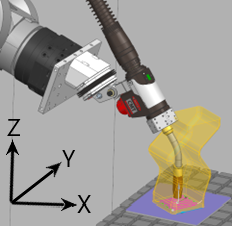
\includegraphics[width=.4\textwidth]{figures/rot0.png} }}%
	\qquad
	\subfloat[\centering 30 degree rotation]{{ 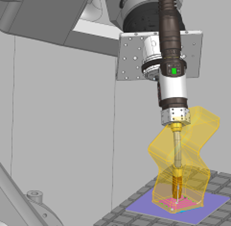
\includegraphics[width=.4\textwidth]{figures/rot1.png}}}%
	\caption{Rotation around the C-axis of a welding torch }%
	\label{rot}%
\end{figure}
 
To determine how optimal the pose of the robot is for the cables it is necessary to know additional parameters. 
In some cases, the cable routing is preferably in a certain orientation along a vector in space and can be translated parallel in direction of that vector. in this case that angle between the planes of the base coordinate system of the robot is constant. 


In other cases it is most optimal for the routing to bo directed towards a specific point in space. This can for example a mounting point of the cables on a wall.  


\begin{figure}[H]%
	\centering
	\subfloat[\centering XXX]{{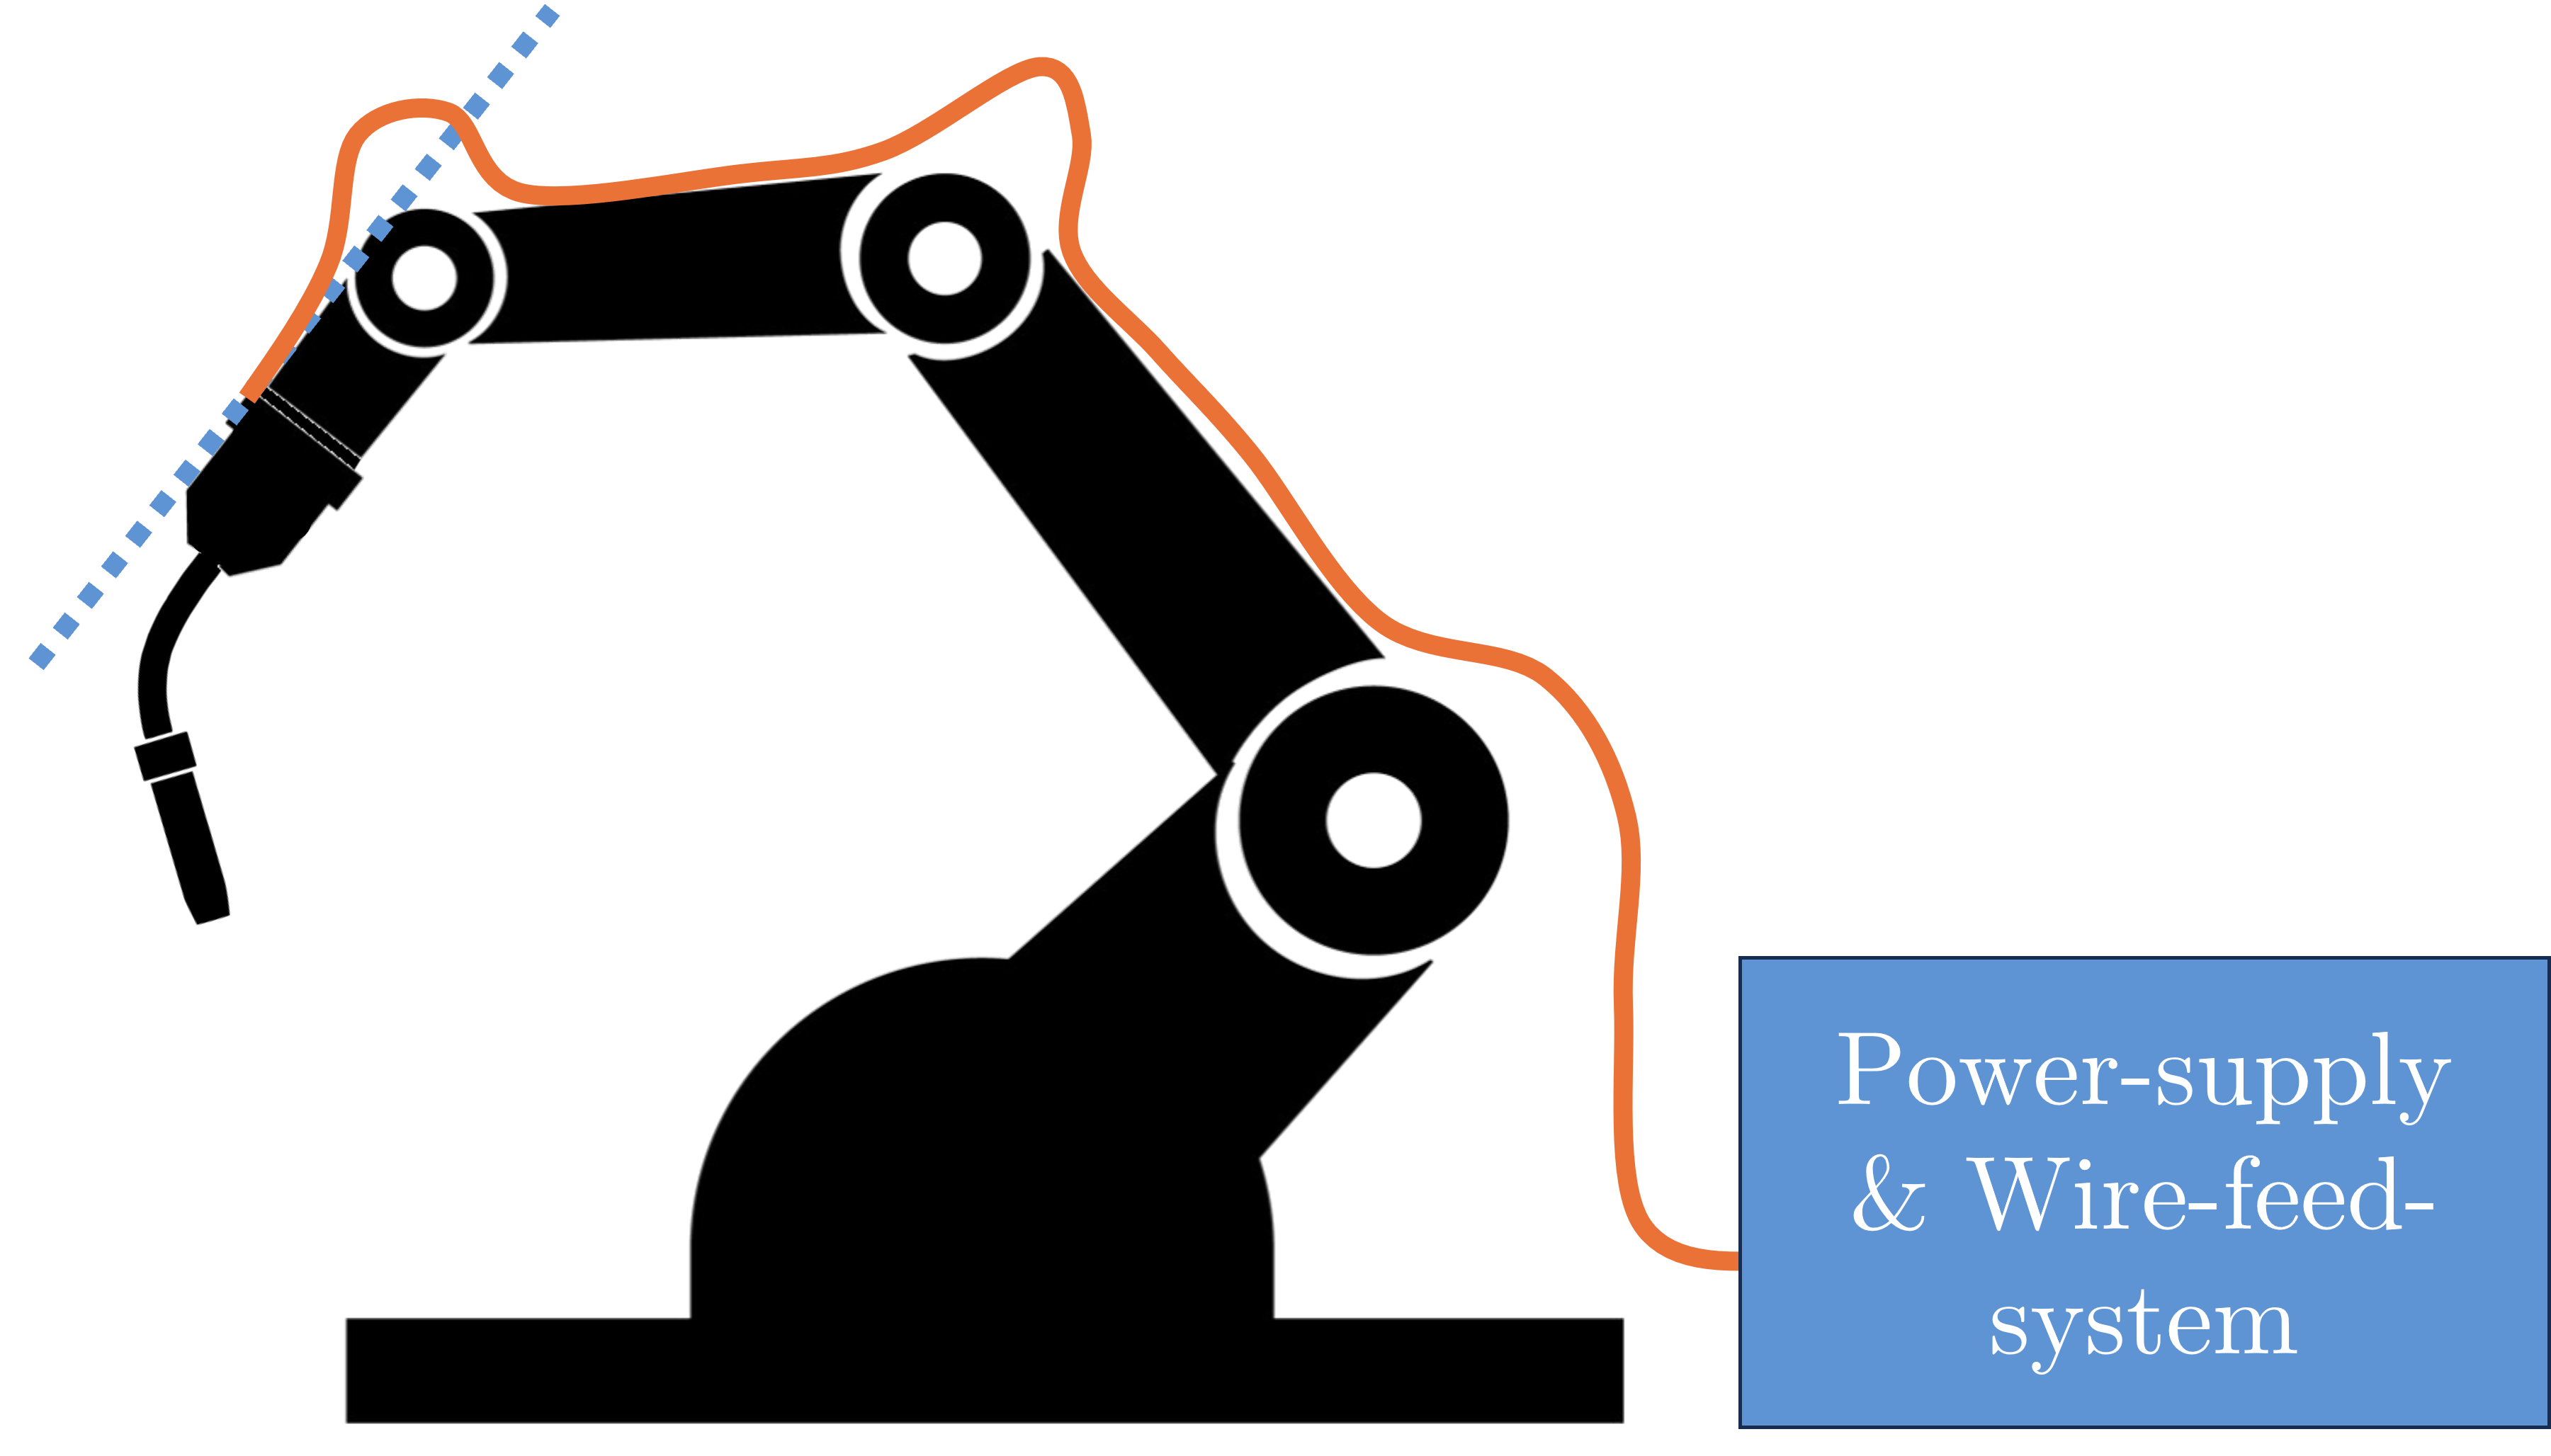
\includegraphics[width=.4\textwidth]{figures/paralell.png} }}%
	\qquad
	\subfloat[\centering XX]{{ 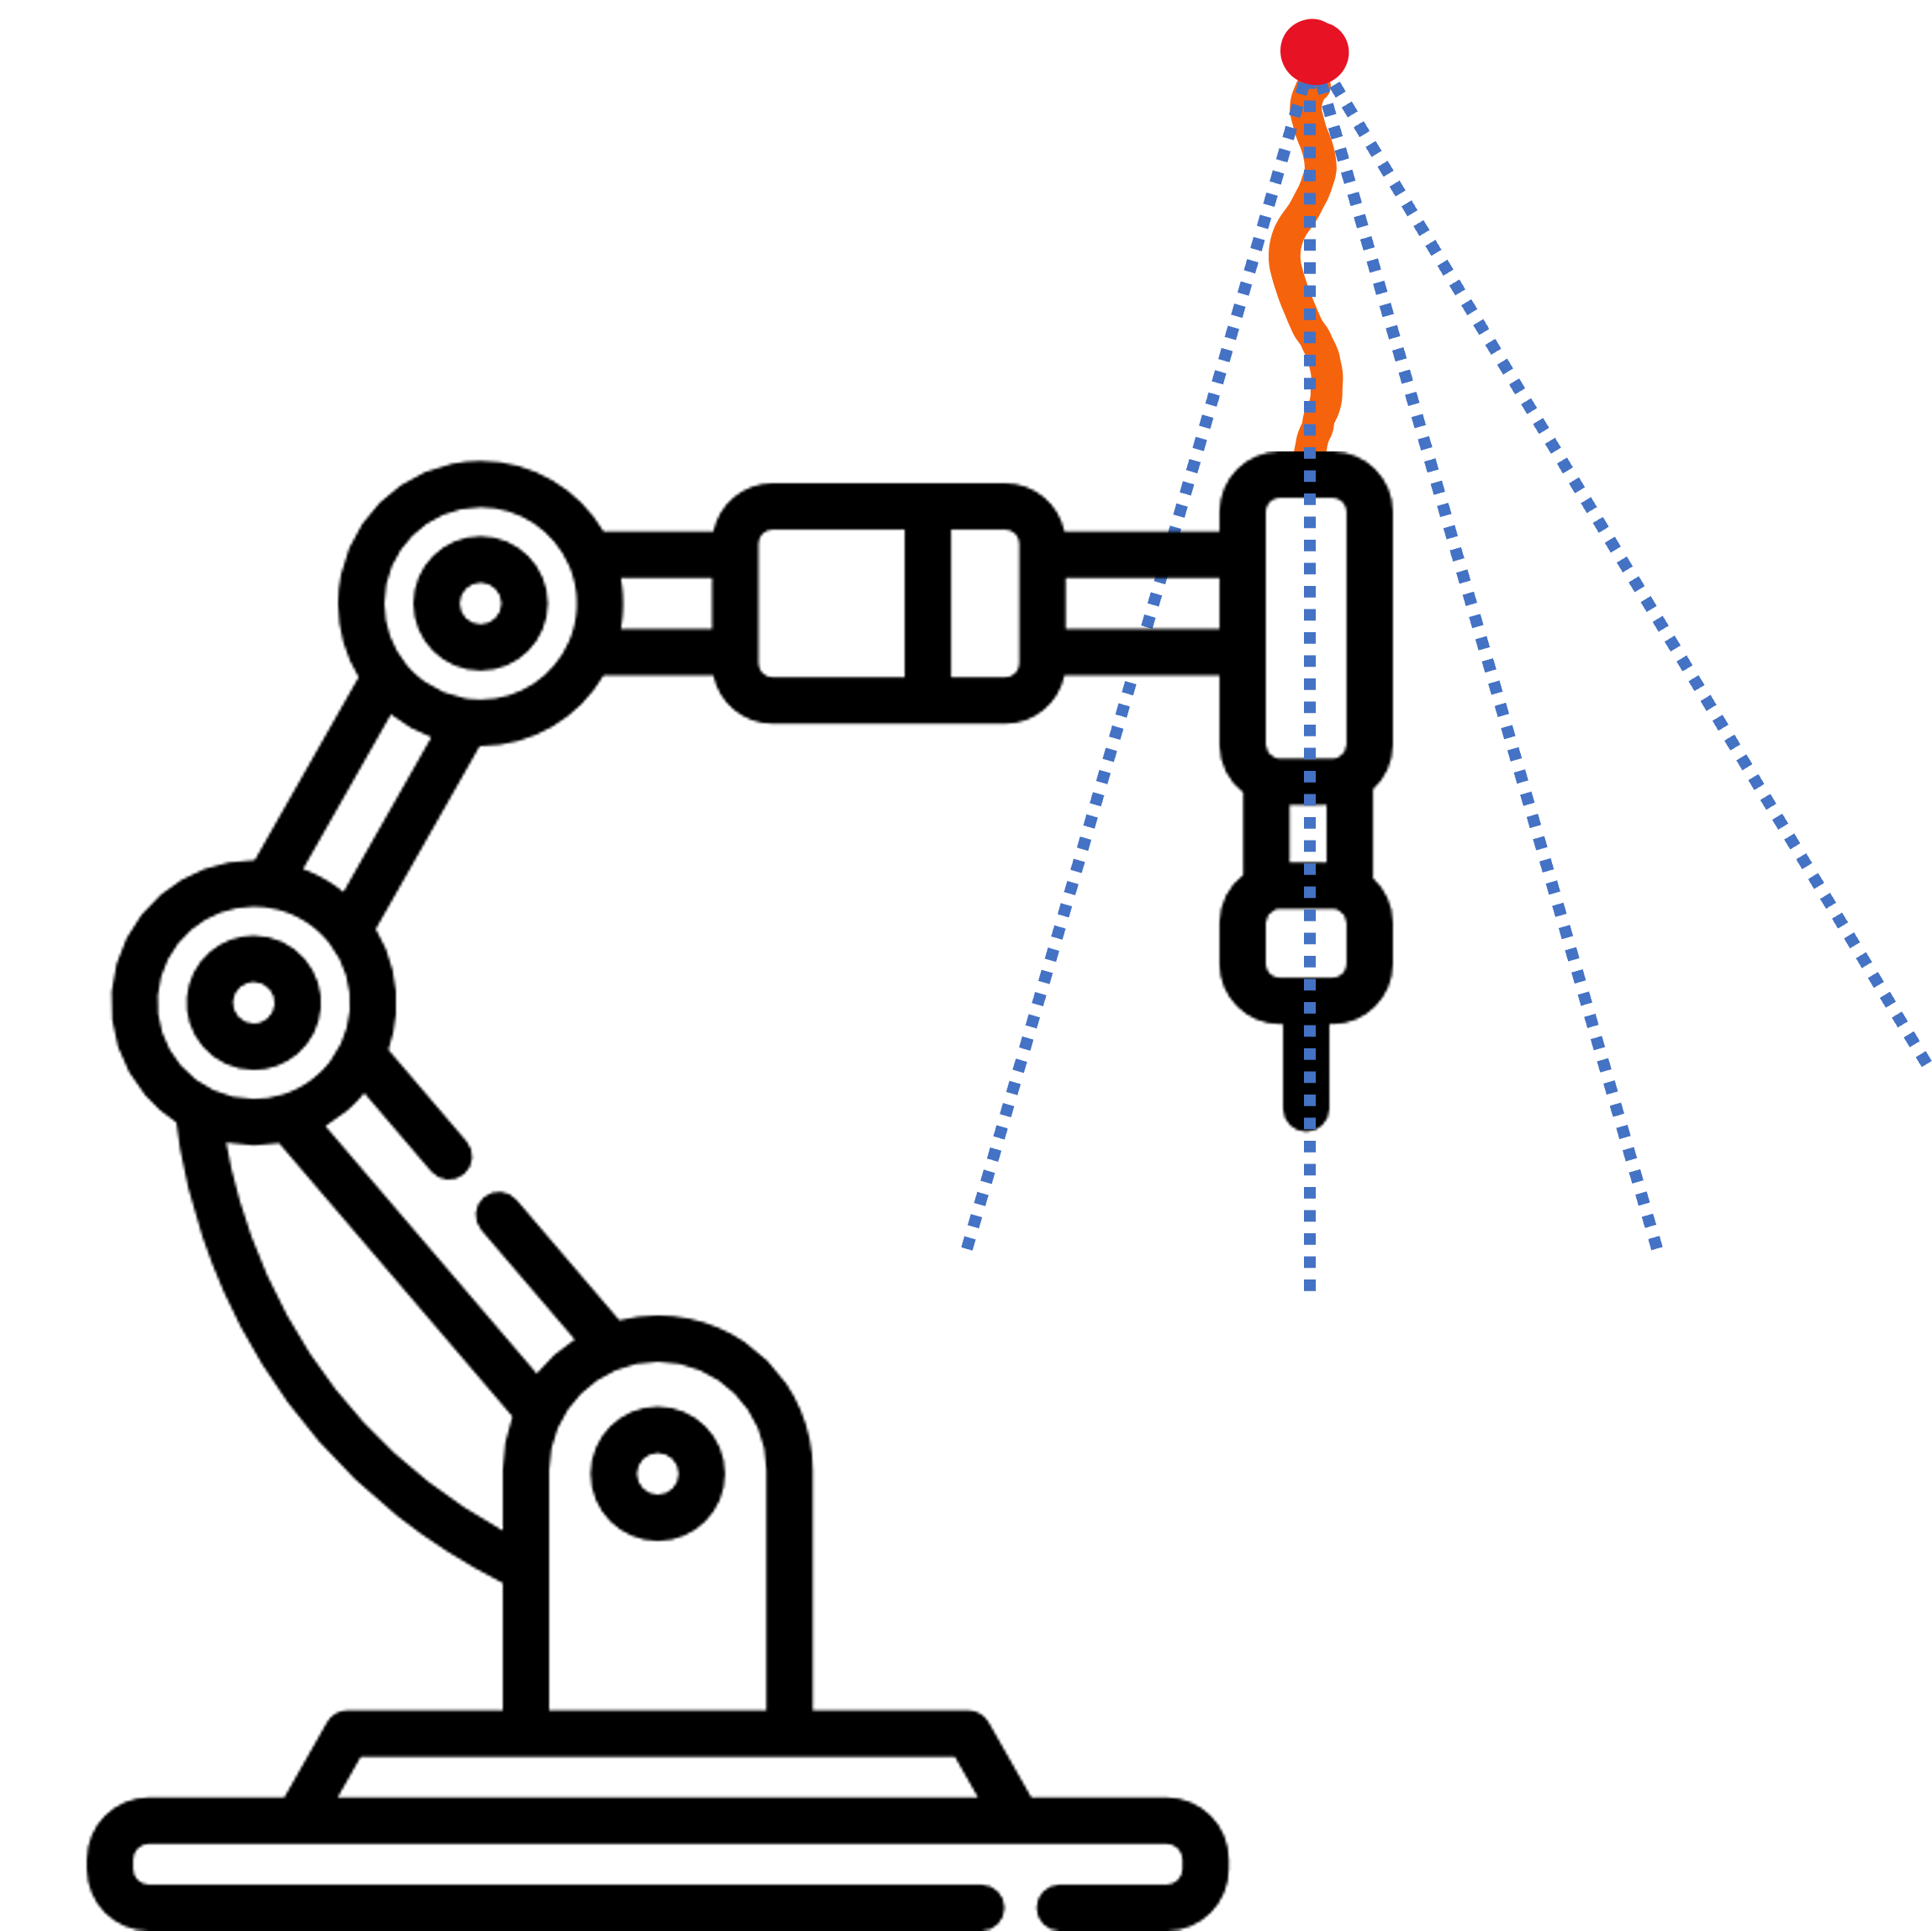
\includegraphics[width=.4\textwidth]{figures/angle.png}}}%
	\caption{ss }%
	\label{sss}%
\end{figure}


\subsection{Singularities }
\subsection{Torch Orientation}
\section{Summery for Boundary Condition Evaluation}
\section{General Methodology for Process Optimization}
\subsection{Without NX}
\subsection{With NX}